%%%%%%%%%%%%%%%%%%%%%%%%%%%%%%%%%%%%%%%%%%%%%%%%%%%%%%%%
%%%%%%%%%%%%%%%%%%%%%%%%%%%%%%%%%%%%%%%%%%%%%%%%%%%%%%%%
\section[SM]{The Standard Model and beyond}
\setcounter{tocdepth}{2}

\begin{frame}
\begin{center}
The Standard Model and beyond
\end{center}
\end{frame}

\subsection{SM}
\begin{frame}{The Standard Model}
\vspace{-.2cm}
\begin{columns}

\begin{column}{.50\textwidth}
\begin{block}{}
\begin{itemize}\scriptsize
%\item Theory developed from quantum theory and special relativity -> Quantum Field Theory (Feynman, Dirac, ...) + Continuous group symmetries (Noether, Yang, ...)
\item Model developed from quantum theory and special relativity $\to$ Quantum Field Theory + Continuous group symmetries
\item Fermions: matter components (electron, muon, quarks...)
\item Bosons: interaction mediators (\W, \Z, ...)
\item Extremely successful model: \\ quarks, CKM, \W~and \Z~masses, ...
\item But it is limited:
  \begin{itemize}\scriptsize
  \item Neutrino masses
  \item Dark matter
  \item \textbf{Hierarchy problem}
  \end{itemize}
\end{itemize}
\end{block}
\end{column}

\begin{column}{.50\textwidth}
\begin{figure}[!Hhtbp]
  \begin{center}
    \includegraphics[width=1.0\textwidth]{../figs/Standard_Model_of_Elementary_Particles.jpg}\\
    \vspace{.6cm}
    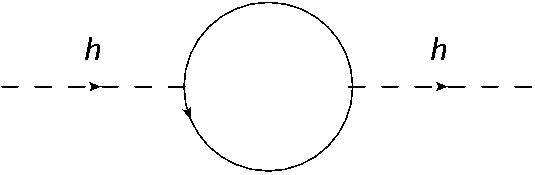
\includegraphics[width=0.8\textwidth]{../figs/HierarchyLoop.png}
    %\caption{Particle content of the standard model.}
    %\label{fig:SMContent}
  \end{center}
\end{figure}
\end{column}
\end{columns}
\end{frame}


\begin{frame}{Vector Like Quarks (VLQ)}
\vspace{-.3cm}
\begin{columns}

\begin{column}{.50\textwidth}
\begin{block}{}
\begin{itemize}\scriptsize
\item Motivated by the hierarchy problem $\to$ New states to cancel loop contributions
\item SM + not chiral quarks
\item Singlet, doublet or triplet representations.
  \begin{itemize}\scriptsize
  \item $X$ with 5/3 electric charge
  \item \textbf{\Tp~with 2/3 electric charge, as the top quark.}
  \item $B$ with -1/3 electric charge, as the bottom quark.
  \item $Y$ with -4/3 electric charge.
  \end{itemize}
%\item \textbf{Generically they can be mixed with the three SM-quark generations}
%\item Produced in pairs or in single production mode with a SM-quark
%\item $T'\to bW^{+/-}, tZ^{0}, tH^{0}$
\end{itemize}
\end{block}
\end{column}

\begin{column}{.50\textwidth}
\begin{figure}[!Hhtbp]
  \begin{center}
    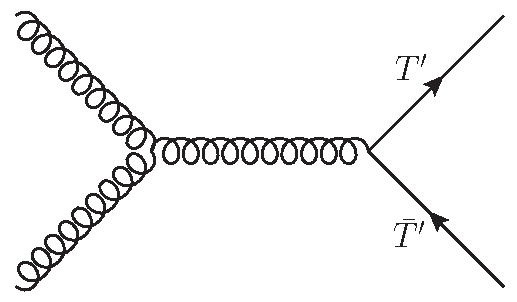
\includegraphics[width=0.5\textwidth]{../figs/Gluon_fusion_T_pair.jpg}
    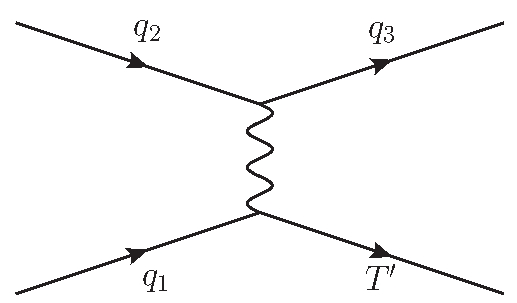
\includegraphics[width=0.5\textwidth]{../figs/Tchannel_T_single.jpg}
  \end{center}
\end{figure}
\vspace{-.2cm}
\begin{block}{}
\begin{itemize}\scriptsize
\item \textbf{Generically they can be mixed with the three SM-quark generations}
\item Produced in pairs or in single production mode with a SM-quark
\item $T'\to bW^{+/-}, tZ^{0}, tH^{0}$
\end{itemize}
\end{block}

\end{column}
\end{columns}

\vspace{-.2cm}
\begin{figure}[!Hhtbp]
  \begin{center}
    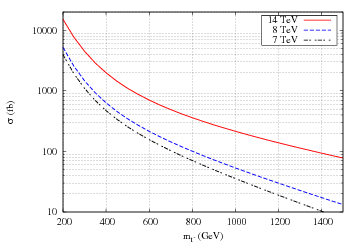
\includegraphics[width=0.4\textwidth]{../figs/pheno_prod_single_tp.png}
    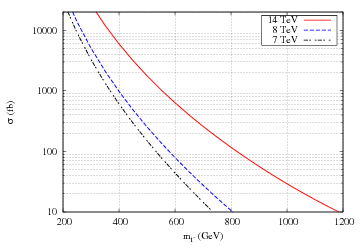
\includegraphics[width=0.4\textwidth]{../figs/pheno_prod_pair_tp.png}
  \end{center}
\end{figure}

\end{frame}

\begin{frame}{SM at the LHC}
\vspace{-.3cm}
\begin{columns}

\begin{column}{.50\textwidth}
\begin{block}{Top quark production}
\begin{itemize}\tiny
\item Heaviest quark in the SM 
\item LHC as a top machine $\to$ 6 tops/s (5 from pair, 1 from single)
\item 8 TeV: $\sigma_{t\bar{t}}=247.47\pm12.37$ pb, $\sigma_{t,\; \text{s-channel}}=5.56\pm0.22$ pb, $\sigma_{t,\; \text{t-channel}}=84.34\pm1.69$ pb and $\sigma_{tW}=22.2\pm0.67$ pb
\item $t\to bW^{-}$ with $Br(W^{+/-}\to l\nu)=0.33$ and $Br(W^{+/-}\to q\bar{q}')=0.67$
\item $m_{t}=173.34\pm 0.76$ \GeVcc
\end{itemize}
\end{block}

\vspace{-.4cm}
\begin{figure}[!Hhtbp]
  \begin{center}
    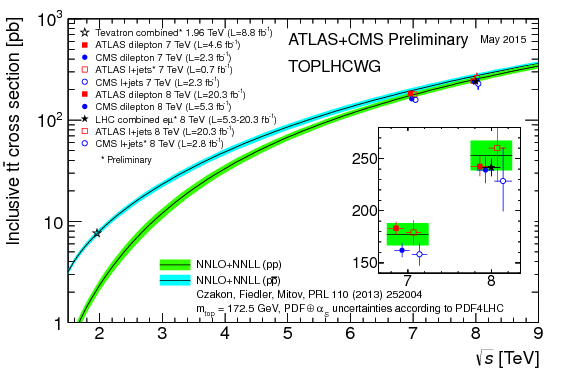
\includegraphics[width=1.0\textwidth]{../figs/toplhcwg_ttxsec_sqrts_may2015.png}
    %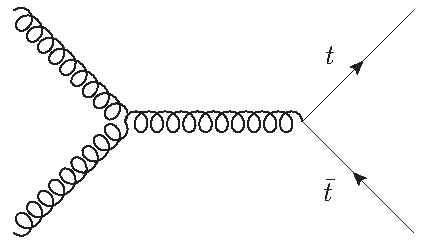
\includegraphics[width=0.3\textwidth]{../figs/Gluon_fusion_top_pair.jpg}
  \end{center}
\end{figure}
\end{column}

\begin{column}{.50\textwidth}
\begin{block}{Higgs boson production}
\begin{itemize}\tiny
\item Heaviest boson in the SM 
\item Rare process: 20 pb at 8TeV
\item Many decay channels: $Br(H^{o}\to b\bar{b})=0.57$
\item $m_{H}=125.09\pm 0.24$ \GeVcc~and $\sigma_{H}<20$ MeV
\end{itemize}
\end{block}

\vspace{-.2cm}
\begin{figure}[!Hhtbp]
  \begin{center}
    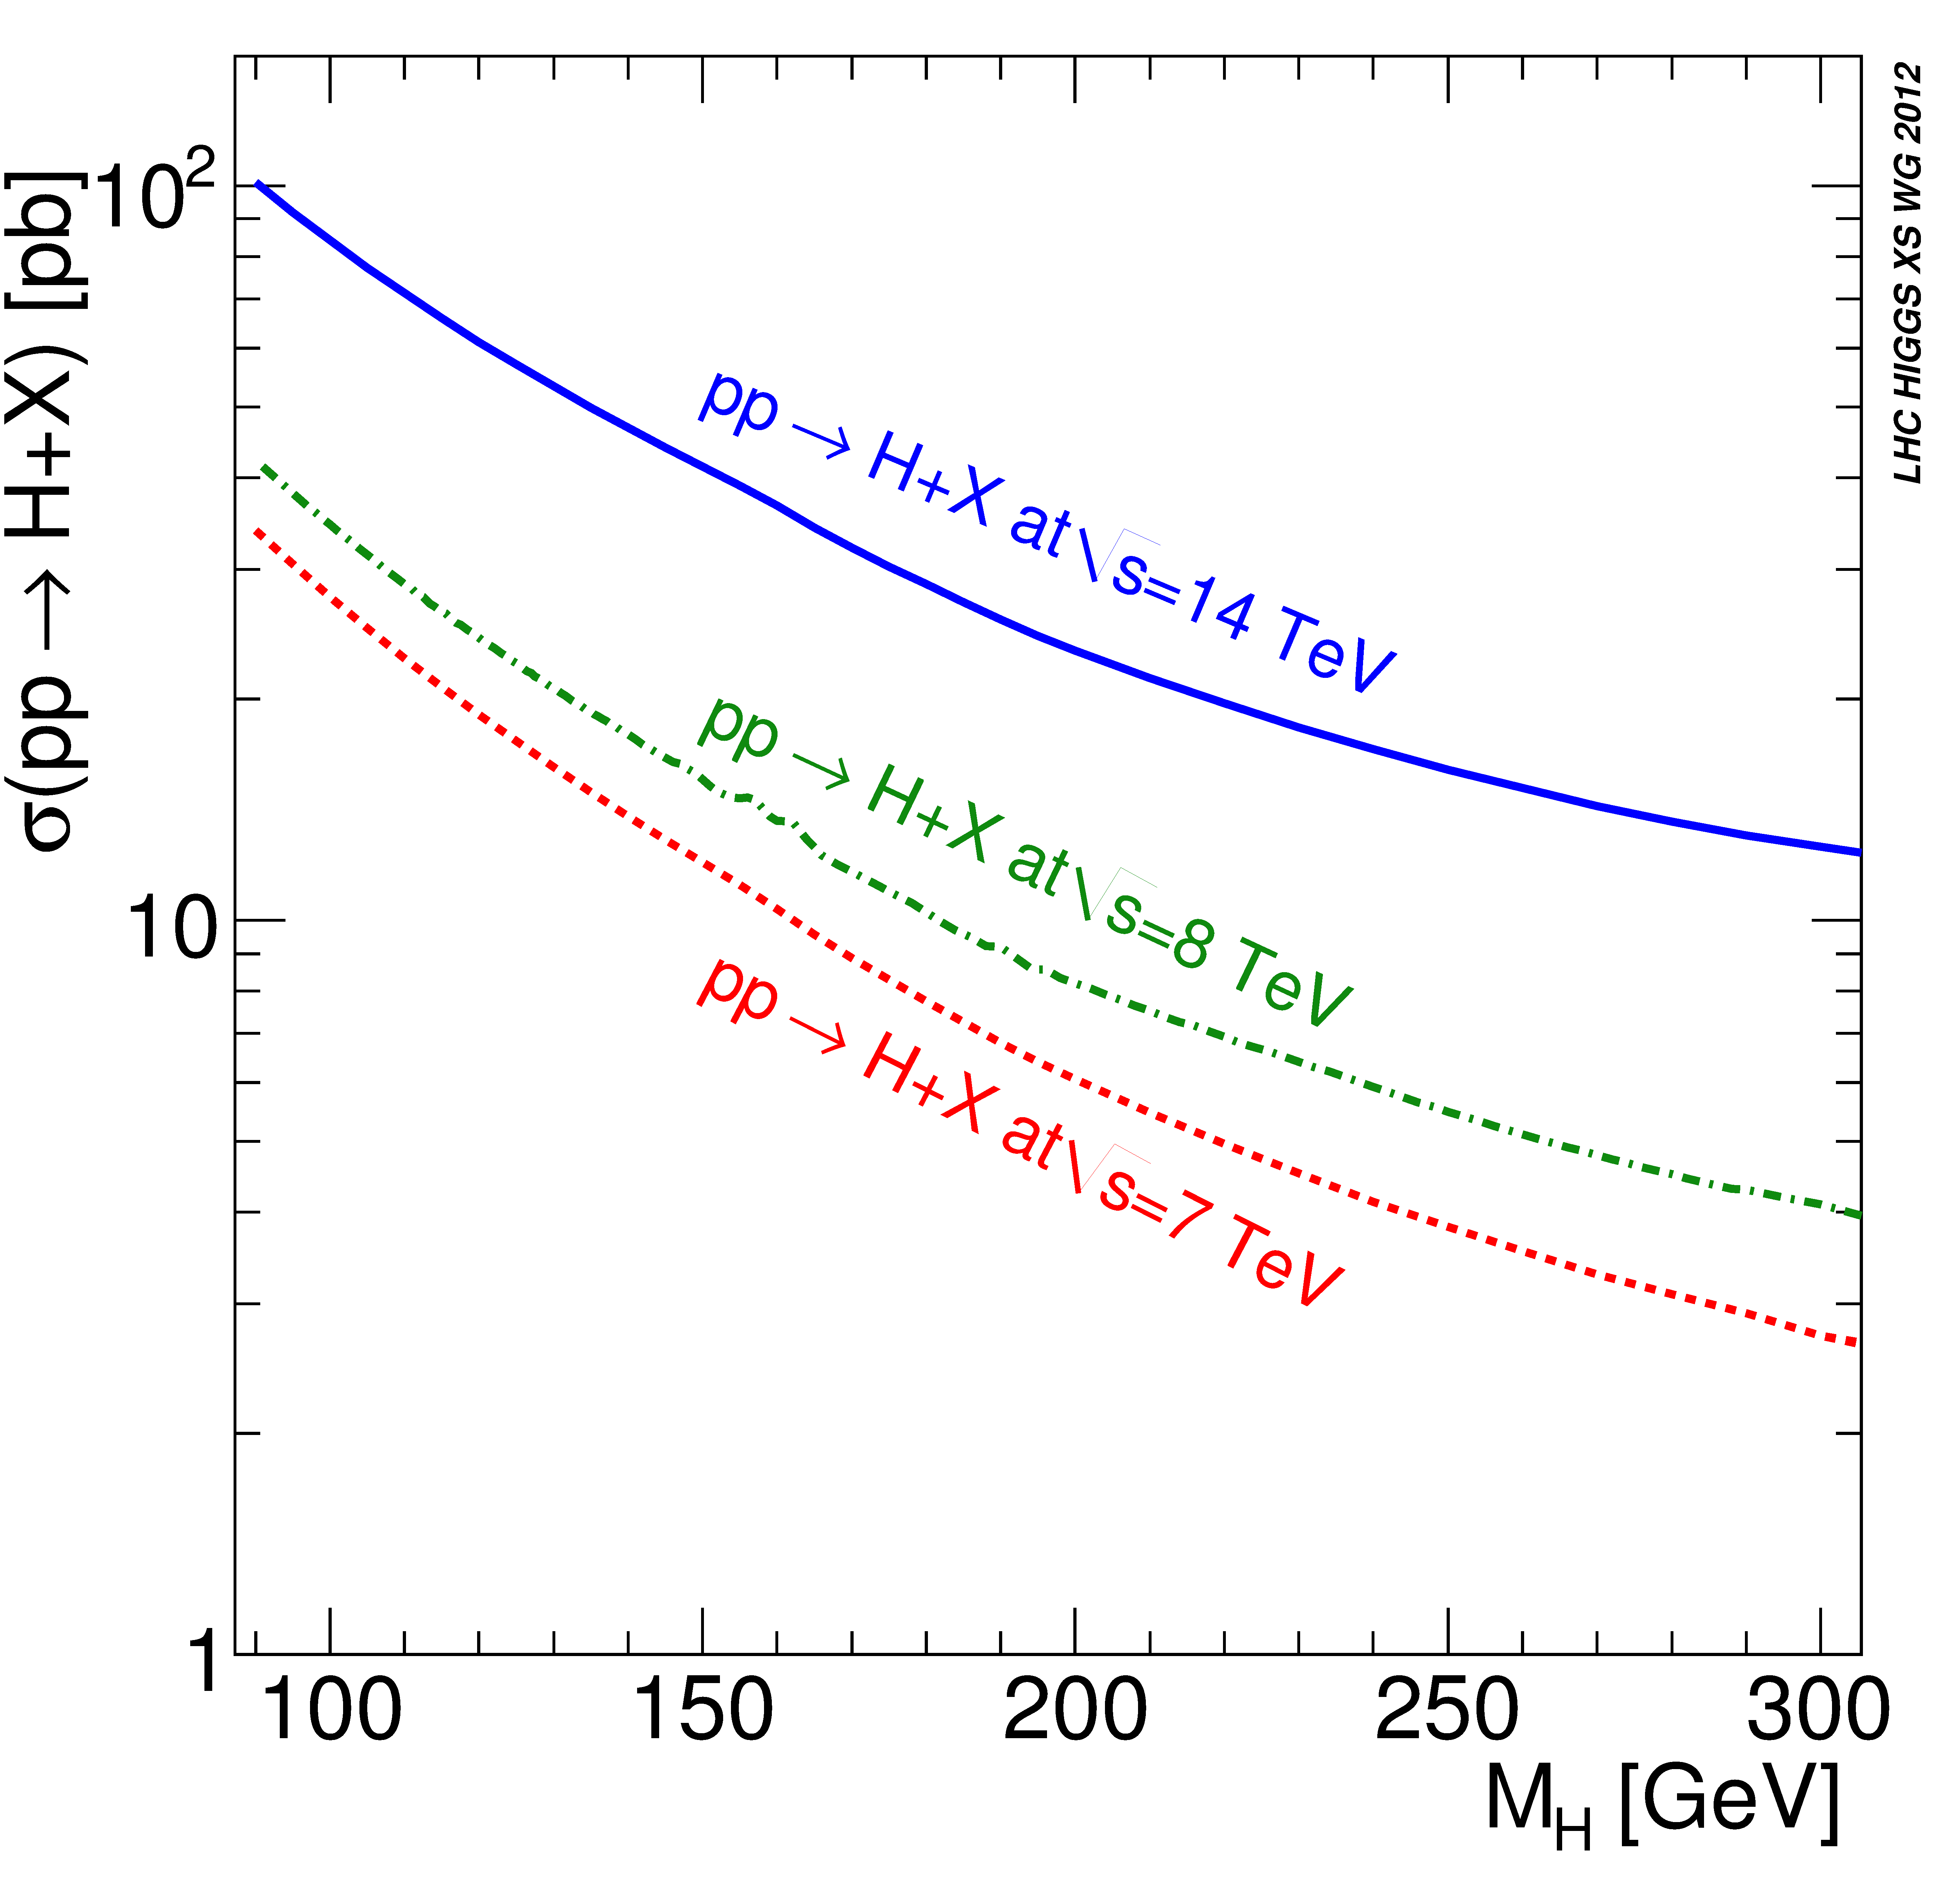
\includegraphics[width=0.8\textwidth]{../figs/totalXS_LM.png}
  \end{center}
\end{figure}

\end{column}
\end{columns}

\end{frame}

